\chapter{Evaluation and Discussion}
\label{cha:discussion}

\section{Evaluation}
\label{sec:evaluation}
\begin{comment}

When evaluating your results, avoid drawing grand conclusions, beyond those that your results can in fact support.
Further, although you may have designed your experiments to answer certain questions,
the results may raise other questions in the eyes of the reader.
It is important that you study the graphs/tables to look for unusual features/entries, and discuss these as well as the main findings.
In particular, carry out an error analysis: What went wrong and why?

A confusion matrix can, for example, be a good way to display misclassifications.
Figure~\ref{fig:conf_sentiment} (on Page~\pageref{fig:conf_sentiment}) shows two confusion matrices.
If there were perfect correlation between true and predicted labels, the long diagonals (from the upper left to the lower right corner) would be completely red.
However,  the confusion matrices indicate
that this classifier was quite biased towards the neutral label (illustrated with \Neutrey),
as can be seen from the warm colours in the positive (\Smiley) and negative (\Sadey) true label cells of the \Neutrey predicted label column.

% Axis configuration for confusion matrices with pgfplots
\pgfplotsset{
    colormap={whitehot}{color(0cm)=(white); color(1cm)=(yellow); color(2cm)=(orange); color(3cm)=(red)},
    confusionaxis/.style={
            colorbar,
            colorbar style={
                    width=2mm,
                    at={(1.05,1)},
                },
            colormap name=whitehot,
            faceted color=none, % remove lines between fields
            view={0}{90},
            y dir=reverse,
            xlabel=Predicted label,
            ylabel=True label,
            tick style={draw=none},
            yticklabels={,,},
            xticklabels={,,},
            every node=[font=\small],
            extra x ticks={0.4,1.5,2.6},
            extra x tick labels={\Smiley, \Neutrey, \Sadey},
            extra y ticks={0.3,1.5,2.7},
            extra y tick labels={\Smiley, \Neutrey, \Sadey},
            extra x tick style={
                    x tick label style={
                            font=\Large
                        }
                },
            extra y tick style={
                    y tick label style={
                            font=\Large
                        }
                },
            width=.4\linewidth,
        }
}

\begin{figure}[t!]
    \centering
    \begin{subfigure}{\linewidth}
        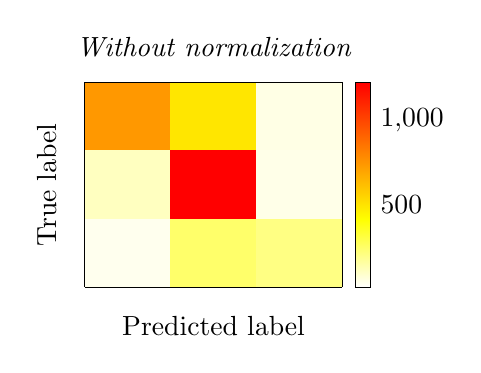
\begin{tikzpicture}
            \begin{axis}[
                    confusionaxis,
                    title={\em Without normalization},
                ]
                \addplot3
                [surf,mesh/cols=4,shader=flat corner
                ] coordinates {
                        (0,0,740) (1,0,490 ) (2,0,43 ) (3,0,1)
                        (0,1,102) (1,1,1229) (2,1,38 ) (3,1,1)
                        (0,2,28 ) (1,2,240 ) (2,2,199) (3,2,1)
                        (0,3,1  ) (1,3,1   ) (2,3,1  ) (3,3,1)
                    };
            \end{axis}
        \end{tikzpicture}
        %\hfill
        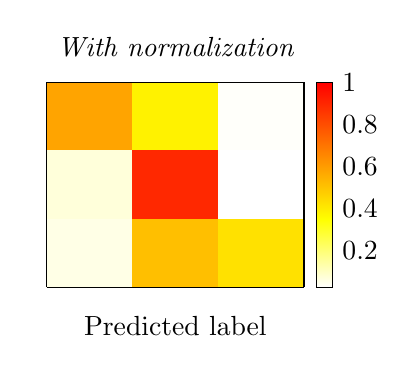
\begin{tikzpicture}
            \begin{axis}[
                    confusionaxis,
                    title={\em With normalization},
                    ylabel={},
                    colorbar style={
                            ylabel={},
                            yticklabel style={
                                    align=right,
                                }
                        },
                ]
                \addplot3
                [surf,mesh/cols=4,shader=flat corner
                ] coordinates {
                        (0,0,0.58130401) (1,0,0.38491752) (2,0,0.03377848) (3,0,1)
                        (0,1,0.07450694) (1,1,0.89773557) (2,1,0.02775749) (3,1,1)
                        (0,2,0.05995717) (1,2,0.51391863) (2,2,0.4261242 ) (3,2,1)
                        (0,3,1         ) (1,3,1         ) (2,3,1         ) (3,3,1)
                    };
            \end{axis}
        \end{tikzpicture}
        \label{fig:conf_sentiment_2013}
    \end{subfigure}
    \caption{Sentiment classifier confusion matrices}
    \label{fig:conf_sentiment}
\end{figure}

\end{comment}
\section{Discussion}
\label{sec:discussion}
\begin{comment}

In this section it is important to include a discussion of not just the merits of the work conducted, but also the limitations.
Which choices did you make? Why? What alternatives were there?
{\color{red}\textbf{Note that a key part of the Master's Thesis grading is based on the student's ability to discuss the results in light of the work by others as well as the restrictions and potential of the work itself.}}
While the Results section will report the outcome of each specific experiments, the Discussion should put those results into perspective and look at overall lessons that can be learned from the entire series of experiments.

You should be able to discuss your work in relation to its overall goal and your research questions (i.e., those introduced in Chapter~\ref{cha:introduction}),
but also address issues such as any ethical considerations that the work may entail,
as well as its technical challenges and limitations.

Discussion and evaluation can either be two different chapters, a joint chapter (as here), or part of the concluding chapter
--- or the discussion can be part of that chapter while the evaluation is part of the experimental chapter.

As for most parts of the thesis, it is possible to select various outlines and setups for the discussion; the important thing is that all the relevant parts appear \textit{somewhere\/} in the text.
\end{comment}

\subsection[Difficulties with OGC API Features]{Difficulties with \acrshort{acr:ogc} \acrshort{acr:api} Features}

A common source of error with several of the tests conducted with the \acrshort{acr:ogc} \acrshort{acr:api} Features agent in was its inability to fetch more than 10,000 features from the server. The limit of 10,000 features is specified in the Features standard \citep{opengeospatialconsortiumOGCAPIFeatures2022}, meaning that no more than 10,000 features should be returned in a single response. Accompanied by such a large response, however, should be a \texttt{next} link than should point to the next set of 10,000 features. This way, the server could return more than 10,000 features. Unfortunately, as of \today, the current version of \textit{pg\_featuresserv} does not support this features\footnote{\url{https://github.com/CrunchyData/pg_featureserv/blob/master/FEATURES.md}}, which is a significant limitation to the current \acrshort{acr:ogc} \acrshort{acr:api} Features implementation for GeoGPT.

Furthermore, the lack of multi-collection queries is in the author's opinion a big limitation to the current Features specification. A proposal draft\footnote{\url{https://github.com/opengeospatial/ogcapi-features/tree/master/proposals/search}} to such features have been created, but it is unclear whether this will accepted into the specification. This extension, called \textit{Search}, would allow for more complex \acrshort{acr:cql} queries than are not easily specified using query parameters. \autoref{code:multi-collection-cql} shows one of the multi-collection query examples included in the proposal draft. Being able to construct such queries could make retrieval of features much more efficient, possibly making the Python tool in the current GeoGPT implementation redundant. This query would not be possible using the current implementation, and one would have to download the two collections, load them into memory using Python, and perform the \texttt{contains} operation there. Being able to construct such \acrshort{acr:cql} queries would offload this work to the Features server which (if the data source is a PostGIS database) would run very efficient \acrshort{acr:sql} code instead of the less than optimal Python code that would otherwise be necessary.

\begin{lstlisting}[
    caption=Multi-collection CQL query using the \textit{Search} extension,
    label=code:multi-collection-cql
]
\\ SQL query for fetching lakes within Algonquin Park
SELECT lakes.*
FROM lakes
JOIN parks ON ST_Intersects(lakes.geometry, parks.geometry)
WHERE parks.name = 'Algonquin Park';

\\ Corresponding CQL query (would return a tuple of parks and lakes)
POST /search   HTTP/1.1                                           
Host: www.someserver.com/                                         
Accept: application/json                                          
Content-Type: application/ogcqry+json                             
                                                                    
[                                                                 
    {                                                              
        "collections": ["parks","lakes"]                            
        "filter": {                                                 
            "and": [                                                 
            {"eq": [{"property": "parks.name"},"Algonquin Park"]} 
            {"contains": [{"property": "parks.geometry"},         
                            {"property": "lakes.geometry"}]}        
            ]                                                        
        }                                                           
    }                                                              
]
\end{lstlisting}


\subsection{Multi-Agent Architectures}